\documentclass[12pt]{article}
\usepackage{amsmath}
\usepackage{amssymb}
\usepackage[letterpaper,margin=0.85in,centering]{geometry}
\usepackage{fancyhdr}
\usepackage{enumerate}
\usepackage{lastpage}
\usepackage{multicol}
\usepackage{graphicx}

\reversemarginpar

\pagestyle{fancy}
\cfoot{}
\lhead{Math 1410}\chead{Worksheet \# 3 Solutions}\rhead{September 28/29, 2016}
%\rfoot{Total: 10 points}
%\chead{{\bf Name:}}
\newcommand{\points}[1]{\marginpar{\hspace{24pt}[#1]}}
\newcommand{\skipline}{\vspace{12pt}}
%\renewcommand{\headrulewidth}{0in}
\headheight 30pt

\newcommand{\di}{\displaystyle}
\newcommand{\abs}[1]{\lvert #1\rvert}
\newcommand{\len}[1]{\lVert #1\rVert}
\renewcommand{\i}{\mathbf{i}}
\renewcommand{\j}{\mathbf{j}}
\renewcommand{\k}{\mathbf{k}}
\newcommand{\R}{\mathbb{R}}
\newcommand{\aaa}{\mathbf{a}}
\newcommand{\bbb}{\mathbf{b}}
\newcommand{\ccc}{\mathbf{c}}
\newcommand{\dotp}{\boldsymbol{\cdot}}
\newcommand{\bbm}{\begin{bmatrix}}
\newcommand{\ebm}{\end{bmatrix}}     
\newcommand{\bvm}{\begin{vmatrix}}
\newcommand{\evm}{\end{vmatrix}}     
\DeclareMathOperator{\proj}{proj}              
                  
\begin{document}

 \begin{enumerate}
\item Find the area of the triangle with vertices $P=(2,0,-1)$, $Q=(-3,4,2)$, and $R=(0,-3,1)$.

\bigskip

Consider the vectors
\begin{align*}
 \vec{u} &= \overrightarrow{PQ}=\langle -5,4,3\rangle \text{ and}\\
 \vec{v} &= \overrightarrow{PR}=\langle -2,-3,2\rangle.
\end{align*}
We know that the area of the parallelogram spanned by $\vec{u}$ and $\vec{v}$ is given by $\len{\vec{u}\times\vec{v}}$, and the given triangle is exactly half of this parallelogram. Since
\begin{align*}
 \vec{u}\times\vec{v} &= \bvm 4&3\\-3&2\evm\hat{\imath}-\bvm -5&3\\-2&2\evm\hat{\jmath}+\bvm -5&4\\-2&-3\evm\hat{k}\\[3pt]
 & = (4(2)-3(-3))\hat{\imath}-(-5(2)-3(-2))\hat{\jmath}+(-5(-3)-4(-2))\hat{k}\\
 & = 17\hat{\imath}+4\hat{\jmath}+23\hat{k} = \langle 17,4,23\rangle,
\end{align*}
we have
\[
 A = \frac{1}{2}\len{\vec{u}\times\vec{v}}=\frac{1}{2}\sqrt{(17)^2+4^2+(23)^2}.
\]


 \item Find the point of intersection (if any) of the line $\langle x,y,z\rangle =  \langle 1, -2, 3\rangle+t\langle 3, 5, -1\rangle$ with the plane $x-2y+3z=-6$

\bigskip

If $(x,y,z)$ is a point that lies on both the line and the plane, then we know that (on the one hand)
\begin{equation}\label{a}
 x=1+3t, \quad y=-2+5t, \quad \text{ and } z=3-t,
\end{equation}

since $(x,y,z)$ lies on the line, and (on the other hand)
\begin{equation}\label{b}
 x-2y+3z=-6,
\end{equation}
since $(x,y,z)$ lies on the plane. Substituting \eqref{a} into \eqref{b}, we get
\[
 (1+3t)-2(-2+5t)+3(3-t)=-6,
\]
which simplifies to $-10t+14=-6$, so $-10t=-20$, and thus $t=2$. Plugging this value for $t$ into \eqref{a}, we get
\[
 x = 1+3(2) = 7,\quad y=-2+5(2) = 8, \quad \text{ and } z=3-2=1.
\]
Thus, the point of intersection is $(7,8,1)$. We can verify that this point is indeed on the plane, since $7-2(8)+3(1)=-6$.

\newpage

\item Find the shortest distance from the point $P=(1,3,-2)$ to the line through the point $P_0 = (2,0,-1)$ in the direction of $\vec{v} = \langle 1,-1,0\rangle$. Also find the point $P_1$ on the line that is closest to $P$. {\bf Include a diagram.}

\bigskip

\begin{multicols}{2}
 We label a generic diagram as shown to the right, with the points $P_0$, $P_1$ on the line labelled, as well as the point $P$ not on the line. From the diagram, we can see that the projection of the vector $\overrightarrow{P_0P}$ onto the line (which is the same as the projection of $\overrightarrow{P_0P}$ onto the vector $\vec{v}$, since $\vec{v}$ is parallel to the line) gives us the vector $\overrightarrow{P_0P_1}$: we have $\overrightarrow{P_0P_1} = \proj_{\vec{v}}\overrightarrow{P_0P}$.
\columnbreak

\begin{center}
 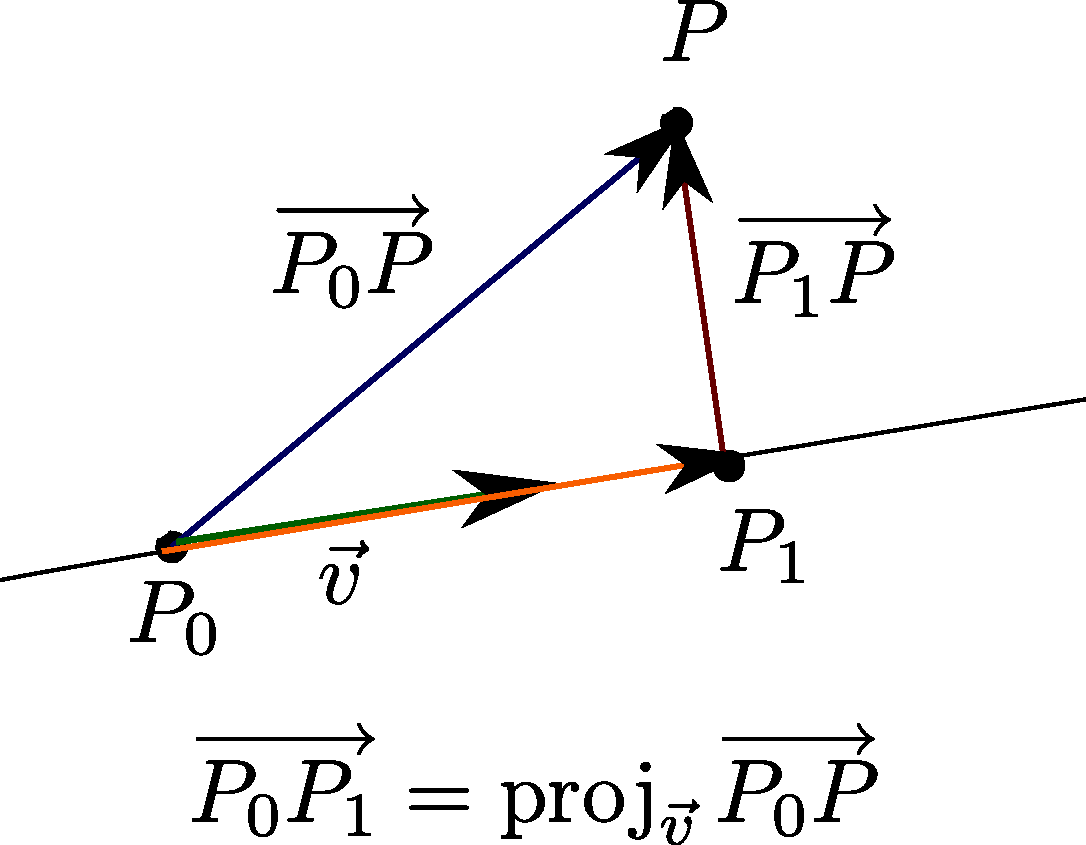
\includegraphics[width=0.7\columnwidth]{WS3-3}
\end{center}
\end{multicols}
We're given $\vec{v} = \langle 1,-1,0\rangle$, and we compute $\overrightarrow{P_0P}=\overrightarrow{OP}-\overrightarrow{OP_0} = \langle 1, 3, -2\rangle-\langle 2, 0, -1\rangle =\langle -1, 3, -1\rangle$. Since $\vec{v}\dotp \overrightarrow{P_0P} = 1(-1)+(-1)(3)+(0)(-1) = -4$ and $\len{\vec{v}}^2 = \vec{v}\dotp\vec{v} = 1^2+(-1)^2+0^2 = 2$, we have
\[
 \overrightarrow{P_0P_1} = \proj_{\vec{v}}\overrightarrow{P_0P} = \left(\frac{\vec{v}\dotp \overrightarrow{P_0P}}{\len{\vec{v}}^2}\right)\vec{v} = \frac{-4}{2}\langle 1, -1, 0\rangle = \langle -2, 2, 0\rangle.
\]
Since $\overrightarrow{P_0P_1} = \overrightarrow{OP_1}-\overrightarrow{OP_0}$, we have
\[
 \overrightarrow{OP_1} = \overrightarrow{OP_0}+\overrightarrow{P_0P_1} = \langle 2, 0, -1\rangle + \langle -2, 2, 0\rangle = \langle 0, 2, -1\rangle,
\]
and thus $P_1 = (0,2,-1)$. Finally, since $P_1$ is the closest point on our line to the point $P$ (as per the diagram above), the distance from the point $P$ to the line is the same as the distance from $P$ to $P_1$. Thus,
\[
 d = d(P,P_1) = \sqrt{(1-0)^2+(3-2)^2+(-2+(-1))^2} = \sqrt{1+1+1}=\sqrt{3}.
\]

{\bf Note:} if we wanted only the distance but didn't need to find the point $P_1$, we can notice (from -- guess what? -- the diagram!) that the distance from the point $P$ to the line is given by the length of the vector $\overrightarrow{P_1P}$, and that 
\[
\overrightarrow{P_1P} = \overrightarrow{P_0P}-\overrightarrow{P_0P_1} = \langle -1, 3, -1\rangle - \langle -2, 2, 0\rangle = \langle 1, 1,  -1\rangle,
\]
and thus $d = \len{\overrightarrow{P_1P}} = \sqrt{1^2+1^2+(-1)^2} = \sqrt{3}$.

\pagebreak


\item Find the shortest distance from the point $P=(2,8,5)$ to the plane given by the equation $x-2y-2z=1$. Also find the point $P_1$ on the plane that is closest to $P$. \\
{\em Hint:} Begin by finding any point $P_0$ that lies on the plane. {\bf Include a diagram.}

\bigskip

\begin{multicols}{2}
We'll give two solutions. The first one uses the hint, along with vectors and projections, as with the previous problem.  We first choose a point on the plane $x-2y-2z=1$. If we set $y=z=0$ in this equation, we're left with $x=1$, so we can take $P_0=(1,0,0)$.  
\columnbreak

\begin{center}
 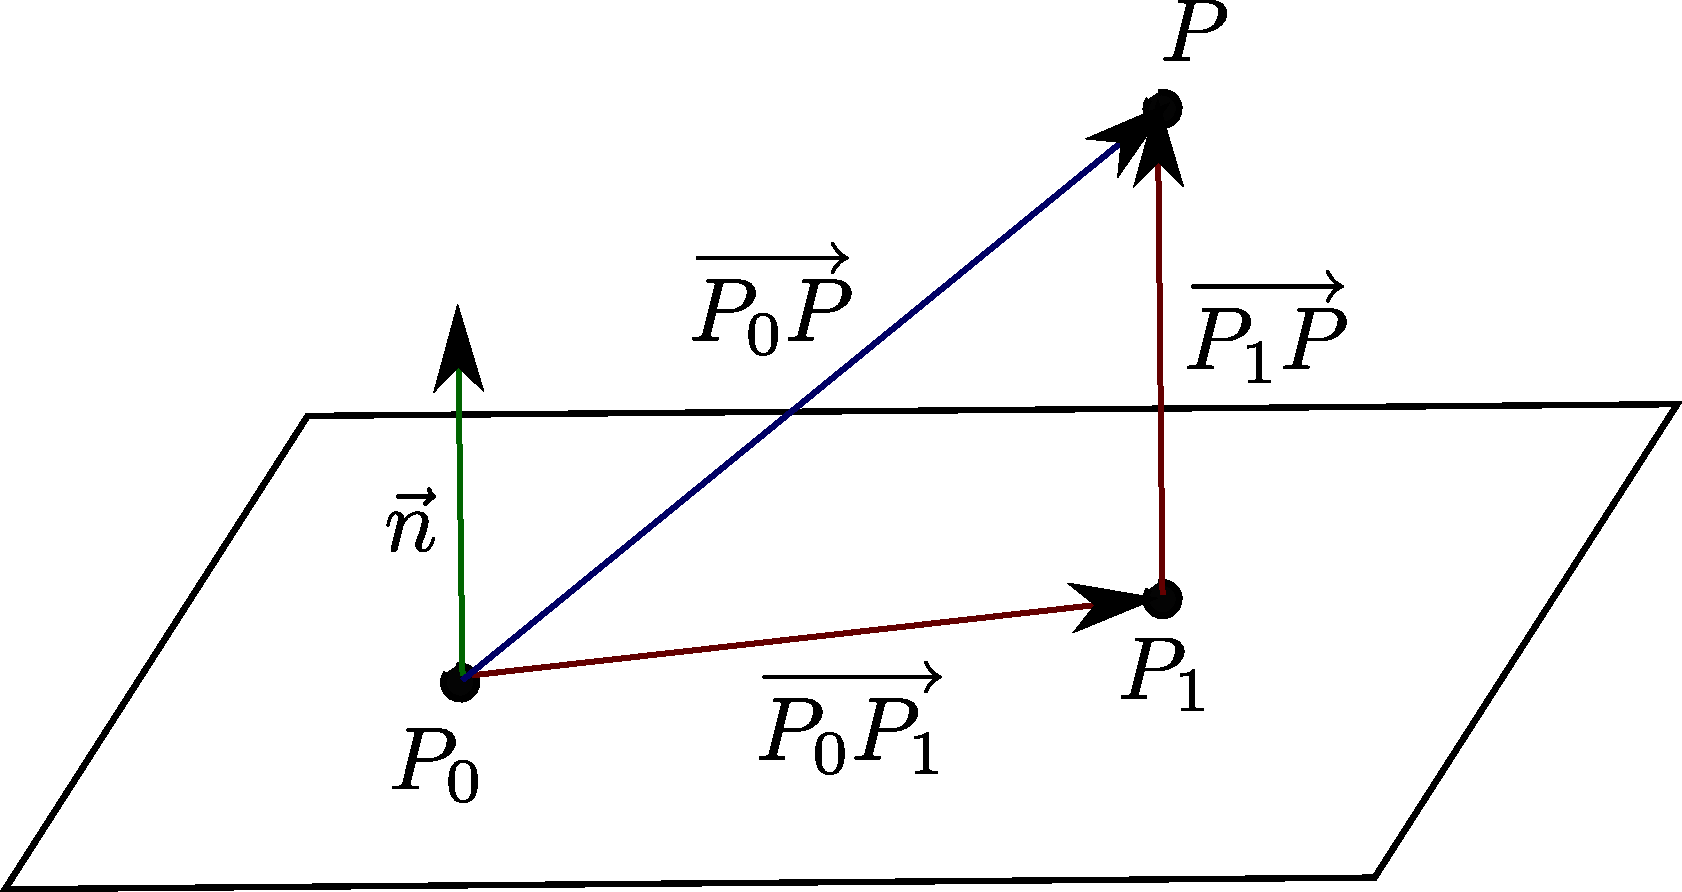
\includegraphics[width=0.8\columnwidth]{WS3-4}
\end{center}
\end{multicols}
Now, referring to the diagram above, we see that the desired distance is given by the length of the vector $\overrightarrow{P_1P}$, where $P_1$ is the point on the plane closest to $P$. Moreover, this vector is the projection of the vector $\overrightarrow{P_0P}$ onto the normal vector $\vec{n}$: $\overrightarrow{P_1P} = \proj_{\vec{n}}\overrightarrow{P_0P}$. (Your answer will not depend on the point $P_0$ that you choose. Changing $P_0$ will change the vectors $\overrightarrow{P_0}$ and $\overrightarrow{P_0P_1}$, but it will not change the vector $\overrightarrow{P_1P}$.)

Recalling that for a general plane $ax+by+cz=d$, the normal vector is given by $\vec{n} = \langle a, b, c\rangle$, we conclude from the equation $x-2y-2z=1$ that our normal vector is $\vec{n} = \langle 1, -2, -2\rangle$. Since we chose $P_0=(1,0,0)$, we have
\[
 \overrightarrow{P_0P} = \overrightarrow{OP}-\overrightarrow{OP_0} = \langle 2, 8, 5\rangle - \langle 1, 0, 0\rangle = \langle 1, 8, 5\rangle.
\]
Since $\vec{n}\dotp\overrightarrow{P_0P} = 1(1)-2(8)-2(5) = -25$ and $\len{\vec{n}} = \sqrt{1^2+(-2)^2+(-2)^2} = \sqrt{9}=3$, we have
\[
 \overrightarrow{P_1P} = \proj_{\vec{n}}\overrightarrow{P_0P} = \left(\frac{\vec{n}\dotp\overrightarrow{P_0P}}{\len{\vec{n}}^2}\right)\vec{n} = \left(\frac{-25}{9}\right)\langle 1, -2, -2\rangle = \langle -25/9, 50/9, 50/9\rangle.
\]
The distance from $P$ to the plane is therefore
\[
 d=\len{\overrightarrow{P_1P}} = \left\lVert \left(\frac{-25}{9}\right)\langle 1, -2, -2\rangle\right\rVert = \frac{25}{9}\left\lVert \langle 1, -2, -2\rangle\right\rVert = \frac{25}{9}(3) = \frac{25}{3}.
\]
To find the point $P_1$, we note that $\overrightarrow{P_1P} = \overrightarrow{OP}-\overrightarrow{OP_1}$, so
\begin{align*}
 \overrightarrow{OP_1} = \overrightarrow{OP}-\overrightarrow{P_1P} &= \langle 2, 8, 5\rangle - \left\langle -\frac{25}{9}, \frac{50}{9}, \frac{50}{9}\right\rangle\\
& = \left\langle 2+\frac{25}{9}, 8-\frac{50}{9}, 5-\frac{50}{9}\right\rangle = \left\langle \frac{43}{9}, \frac{22}{9}, -\frac{5}{9}\right\rangle,
\end{align*}
so $P_1 = \left(\dfrac{43}{9},\dfrac{22}{9},-\dfrac{5}{9}\right)$.

\pagebreak

The second solution is to turn Problem 4 in to Problem 2. Referring again to the diagram above, if we construct the line $L$ that passes through the point $P$ in the direction of the normal vector $\vec{n}$, then the point $P_1$ we're looking for is exactly the point where $L$ intersects the plane $x-2y-2z=1$. As above, we have $\vec{n} = \langle 1, -2, -2\rangle$, so the line $L$ is given by the vector equation
\[
 \langle x, y, z\rangle = \langle 2, 8, 5\rangle + t\langle 1, -2, -2\rangle.
\]
Substituting $x=2+t$, $y=8-2t$, and $z=5-2t$ into the equation $x-2y-2z=1$ of the plane, we have
\[
 (2+t)-2(8-2t)-2(5-2t) = 9t-24=1,
\]
so $9t=25$, and thus $t=\dfrac{25}{9}$. Putting this value for $t$ back into the equations of our normal line through $P$, we get
\[
 P_1 = \left(2+\frac{25}{9},8-\frac{50}{9}, 5-\frac{50}{9}\right) = \left(\frac{43}{9},\frac{22}{9},-\frac{5}{9}\right),
\]
which is the same result we found using the other method. The distance from the point $P$ to the plane is then the same as the distance from $P$ to $P_1$, so using the distance formula we get
\begin{align*}
 d = d(P_1,P) &= \sqrt{\left(2+\frac{25}{9}-2\right)^2+\left(8-\frac{50}{9} - 8\right)^2 + \left(5-\frac{50}{9}-5\right)^2}\\
& = \sqrt{\left(\frac{25}{9}\right)^2+\left(-\frac{50}{9}\right)^2 + \left(-\frac{50}{9}\right)^2}\\
& = \sqrt{\left(\frac{25}{9}\right)^2(1^2+(-2)^2+(-2)^2)}\\
& = \frac{25}{9}\sqrt{1^2+(-2)^2+(-2)^2} = \frac{25}{9}(3) = \frac{25}{3},
\end{align*}
which is the same distance as above.


 \end{enumerate}
\end{document}